\chapter{Chiral Deformation Quantization: From Kontsevich to Chiral Algebras}
\label{ch:chiral-deformation}
\label{chap:chiral-deformation}

\begin{remark}[Epigraph]
\textit{``Deformation quantization is the shadow cast by configuration spaces onto the wall of algebra.''} 

What Kontsevich discovered for Poisson manifolds—that quantization arises from integrating differential forms over configuration spaces—extends naturally to chiral algebras. The operator product expansion is itself a quantization, and the bar-cobar construction provides its geometric realization. This chapter makes this precise.
\end{remark}

\section{Kontsevich's Theorem: The Classical Picture}

\subsection{Statement and Physical Intuition}

Begin with the simplest question: how do we quantize?

Classically, observables form a commutative algebra $C^\infty(M)$ on phase space $M$. A Poisson structure $\{\cdot,\cdot\}$ makes this into a Poisson algebra. Quantum mechanics demands replacing commutative multiplication with a noncommutative product:
$$f \star g = fg + \frac{\hbar}{2}\{f,g\} + \text{higher corrections}$$

The miracle: this deformation exists and is controlled by geometry.

\begin{theorem}[Kontsevich 1997]
Let $(M, \pi)$ be a Poisson manifold with Poisson bivector $\pi \in \Gamma(\wedge^2 TM)$. There exists a star product $\star: C^\infty(M)[[\hbar]] \otimes C^\infty(M)[[\hbar]] \to C^\infty(M)[[\hbar]]$ such that:
\begin{enumerate}
\item $f \star g = fg + \frac{\hbar}{2}\{f,g\} + O(\hbar^2)$
\item $(f \star g) \star h - f \star (g \star h) = 0$ (associativity)
\item The star product is given by an explicit formula:
$$f \star g = \sum_{\Gamma} \frac{\hbar^{|\Gamma|}}{|\text{Aut}(\Gamma)|} w_\Gamma \cdot B_\Gamma(f,g)$$
where the sum is over \emph{directed graphs} $\Gamma$ and $B_\Gamma$ are bidifferential operators constructed by integrating differential forms over configuration spaces.
\end{enumerate}
\end{theorem}

\subsection{The Configuration Space Construction}

The weight $w_\Gamma$ for a graph $\Gamma$ with $n$ vertices is:
$$w_\Gamma = \int_{C_n(\mathbb{H})} \omega_\Gamma$$
where:
\begin{itemize}
\item $C_n(\mathbb{H})$ is the configuration space of $n$ labeled points in the upper half-plane $\mathbb{H} = \{z \in \mathbb{C} : \text{Im}(z) > 0\}$
\item $\omega_\Gamma$ is a differential form constructed from the graph $\Gamma$:
$$\omega_\Gamma = \bigwedge_{e \in E(\Gamma)} d\phi_e$$
where $\phi_e = \arg(z_{\text{target}(e)} - z_{\text{source}(e)})$ is the angle of edge $e$
\end{itemize}

\begin{example}[The First Quantum Correction]
At order $\hbar^2$, there is one graph contributing:
\begin{center}
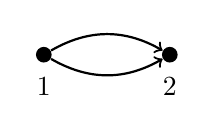
\begin{tikzpicture}[scale=0.8]
\node[circle,fill,inner sep=2pt] (1) at (0,0) {};
\node[circle,fill,inner sep=2pt] (2) at (2,0) {};
\draw[->,thick] (1) to[bend left] (2);
\draw[->,thick] (1) to[bend right] (2);
\node at (0,-0.5) {$1$};
\node at (2,-0.5) {$2$};
\end{tikzpicture}
\end{center}

This contributes:
$$f \star g = fg + \frac{\hbar}{2}\{f,g\} + \frac{\hbar^2}{24}\left(\{\{f,\pi\}, g\} + \{f, \{\pi, g\}\}\right) + O(\hbar^3)$$

The coefficient $\frac{1}{24}$ comes from:
$$w_\Gamma = \int_{C_2(\mathbb{H})} d\phi_{12} \wedge d\phi_{21} = \frac{1}{24}$$
where we use $\phi_{12} = \arg(z_2 - z_1)$ and $\phi_{21} = \arg(z_1 - z_2) = \phi_{12} + \pi$.
\end{example}

\subsection{Why the Upper Half-Plane?}

Witten's insight: The upper half-plane $\mathbb{H}$ is the \emph{simplest example} of a worldsheet.

\begin{itemize}
\item Boundary: The real axis $\mathbb{R} \subset \partial\mathbb{H}$ represents the ``past''
\item Interior: Quantum fluctuations occur in $\mathbb{H}$
\item Asymptotic completeness: Points escaping to infinity represent physical states
\item Conformal symmetry: $\text{PSL}(2,\mathbb{R})$ acts on $\mathbb{H}$ by Möbius transformations
\end{itemize}

The key geometric fact:
$$\overline{C}_n(\mathbb{H})/\text{PSL}(2,\mathbb{R}) = \overline{\mathcal{M}}_{0,n+1}$$
Configuration spaces on $\mathbb{H}$ modulo symmetry give the moduli space of rational curves with marked points!

\section{Chiral Algebras as Quantum Observables}

\subsection{From Poisson to Chiral}

Now replace the Poisson manifold with a curve $X$. The analog of a Poisson structure is a \emph{chiral Poisson structure}.

\begin{definition}[Chiral Poisson Algebra]
A chiral Poisson algebra on a smooth curve $X$ is a sheaf $\mathcal{A}$ of $\mathcal{D}_X$-modules with:
\begin{enumerate}
\item A commutative product (pointwise multiplication of functions)
\item A Poisson bracket $\{\cdot, \cdot\}: \mathcal{A} \boxtimes \mathcal{A} \to \mathcal{A} \otimes \mathcal{D}_X$ satisfying:
$$\{a(z), b(w)\} = \sum_{k=1}^N \frac{P_k(a,b)(w)}{(z-w)^k}$$
where $P_k$ are bidifferential operators
\item Jacobi identity holding ``up to divergence'':
$$\{a, \{b, c\}\} - \{\{a, b\}, c\} - \{b, \{a, c\}\} = \text{(contact terms)}$$
\end{enumerate}
\end{definition}

\begin{example}[Current Algebra]
For a Lie algebra $\mathfrak{g}$, the current algebra $\mathfrak{g}[z]$ has Poisson bracket:
$$\{J^a(z), J^b(w)\} = \frac{f^{abc} J^c(w)}{z-w}$$
This is the \emph{classical limit} of the affine Kac-Moody algebra $\widehat{\mathfrak{g}}_k$ as $k \to \infty$.
\end{example}

\subsection{Operator Product Expansion as Star Product}

The OPE of a chiral algebra is precisely a star product:
$$a(z) \cdot b(w) = \sum_{k=0}^\infty \frac{(a *_k b)(w)}{(z-w)^k}$$

Key observation: This has the same structure as Kontsevich's formula!
\begin{itemize}
\item Classical: $a(z)b(w)$ (commutative product)
\item First quantum: $\frac{\{a, b\}(w)}{z-w}$ (Poisson bracket)
\item Higher quantum: $\frac{(a *_k b)(w)}{(z-w)^k}$ (higher corrections)
\end{itemize}

\begin{theorem}[Chiral Quantization]
Every chiral Poisson algebra admits a canonical quantization to a chiral algebra. The quantization is given by Kontsevich's formula, with $\mathbb{H}$ replaced by the curve $X$.
\end{theorem}

\section{Configuration Space Integrals for Chiral Algebras}

\subsection{The Geometric Setup}

Replace Kontsevich's configuration spaces with chiral configuration spaces:

\begin{definition}[Chiral Configuration Space]
For a smooth curve $X$, define:
$$C_n^{\text{ch}}(X) = C_n(X) \times \prod_{i=1}^n S^1_i$$
where:
\begin{itemize}
\item $C_n(X) = \{(z_1, \ldots, z_n) \in X^n : z_i \neq z_j\}$
\item $S^1_i$ is the circle of \emph{infinitesimal disks} around $z_i$
\item The product encodes both \emph{positions} and \emph{local trivializations}
\end{itemize}

The compactification $\overline{C}_n^{\text{ch}}(X)$ is the Fulton-MacPherson-Ran space.
\end{definition}

\subsection{Forms on Chiral Configuration Spaces}

The differential forms we integrate are \emph{logarithmic forms with coefficients}:

\begin{definition}[Chiral Integration Forms]
On $\overline{C}_n^{\text{ch}}(X)$, define:
$$\Omega^*_{\text{ch}} = \Omega^*_{\text{log}}(\overline{C}_n(X)) \otimes \mathcal{A}^{\boxtimes n}$$
where:
\begin{itemize}
\item $\Omega^*_{\text{log}}$ are logarithmic forms with poles along collision divisors:
$$\eta_{ij} = d\log(z_i - z_j) = \frac{dz_i - dz_j}{z_i - z_j}$$
\item $\mathcal{A}^{\boxtimes n} = \mathcal{A}|_{z_1} \boxtimes \cdots \boxtimes \mathcal{A}|_{z_n}$ are field insertions
\end{itemize}
\end{definition}

\subsection{The Chiral Star Product Formula}

\begin{theorem}[Chiral Kontsevich Formula]
Let $\mathcal{A}_{\text{cl}}$ be a chiral Poisson algebra on $X$. Its quantization $\mathcal{A}_\hbar$ has structure constants:
$$(a \star b)(w) = \sum_{\Gamma \in \mathcal{G}_n} \frac{\hbar^{n}}{|\text{Aut}(\Gamma)|} \int_{\overline{C}_n^{\text{ch}}(X)} B_\Gamma(a,b) \wedge \omega_\Gamma$$
where:
\begin{enumerate}
\item $\mathcal{G}_n$ is the set of admissible graphs with $n$ vertices
\item $B_\Gamma(a,b)$ constructs differential operators from $\Gamma$:
$$B_\Gamma(a,b) = \prod_{v \in V(\Gamma)} \left(\pi_v^{i_v j_v} \frac{\partial}{\partial z_i} \frac{\partial}{\partial w_j}\right) (a(z_v) \otimes b(w_v))$$
\item $\omega_\Gamma$ is the angle form:
$$\omega_\Gamma = \bigwedge_{e \in E(\Gamma)} \frac{dz_{\text{source}(e)} - dz_{\text{target}(e)}}{z_{\text{source}(e)} - z_{\text{target}(e)}}$$
\end{enumerate}
\end{theorem}

\begin{proof}[Idea]
The proof follows Kontsevich's strategy but uses \emph{chiral} structures:

\textbf{Step 1: Formality.}
Show that the $L_\infty$ algebra of polyvector fields $\mathcal{T}_{\text{poly}}^{\text{ch}}(X)$ on $X$ is formal:
$$\mathcal{T}_{\text{poly}}^{\text{ch}}(X) \simeq_{L_\infty} H^*(\mathcal{T}_{\text{poly}}^{\text{ch}}(X))$$

\textbf{Step 2: Configuration space integrals.}
The formality map is given explicitly by:
$$\mathcal{F}_n: \mathcal{T}_{\text{poly}}^{\text{ch}}(X)^{\otimes n} \to \mathcal{T}_{\text{poly}}^{\text{ch}}(X)$$
$$\mathcal{F}_n(\pi_1, \ldots, \pi_n) = \sum_{\Gamma} w_\Gamma \cdot U_\Gamma(\pi_1, \ldots, \pi_n)$$

\textbf{Step 3: Weight computation.}
$$w_\Gamma = \int_{\overline{C}_n^{\text{ch}}(X)} \omega_\Gamma$$

\textbf{Step 4: Star product.}
The star product is recovered by applying $\mathcal{F}$ to the Poisson structure:
$$a \star b = m \circ \exp(\hbar \mathcal{F}(\pi))(a \otimes b)$$
\end{proof}

\section{Explicit Computations Through Degree 5}

\subsection{Organization by Loop Order}

Following Serre's principle: compute everything explicitly in low degrees before abstracting.

\subsubsection{Tree Level ($\hbar^0$): Classical Product}

$$a \star_0 b = ab$$

Graph: Just two vertices, no edges.

\subsubsection{One Loop ($\hbar^1$): Poisson Bracket}

$$a \star_1 b = \frac{1}{2}\{a, b\}$$

Graph: Two vertices with one directed edge $1 \to 2$.

Weight calculation:
$$w = \int_{C_2^{\text{ch}}(X)} d\arg(z_2 - z_1) = \frac{1}{2}$$
(The factor $\frac{1}{2}$ comes from integrating $d\theta$ over $S^1$.)

\subsubsection{Two Loops ($\hbar^2$): First Quantum Correction}

There are three graphs contributing at $\hbar^2$:

\textbf{Graph 1:} Two edges from vertex 1 to vertex 2
\begin{center}
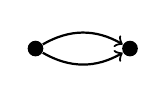
\begin{tikzpicture}[scale=0.6]
\node[circle,fill,inner sep=2pt] (1) at (0,0) {};
\node[circle,fill,inner sep=2pt] (2) at (2,0) {};
\draw[->,thick] (1) to[bend left=30] (2);
\draw[->,thick] (1) to[bend right=30] (2);
\end{tikzpicture}
\end{center}

$$B_{\Gamma_1}(a,b) = \pi^{ij} \pi^{kl} \frac{\partial^2 a}{\partial x^i \partial x^k} \frac{\partial^2 b}{\partial x^j \partial x^l}$$

Weight: $w_{\Gamma_1} = \frac{1}{24}$ (computed via residue formula)

\textbf{Graph 2:} Chain $1 \to 2 \to 1$
\begin{center}
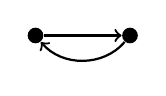
\begin{tikzpicture}[scale=0.6]
\node[circle,fill,inner sep=2pt] (1) at (0,0) {};
\node[circle,fill,inner sep=2pt] (2) at (2,0) {};
\draw[->,thick] (1) -- (2);
\draw[->,thick] (2) to[bend left=50] (1);
\end{tikzpicture}
\end{center}

$$B_{\Gamma_2}(a,b) = \pi^{ij} \pi^{kl} \frac{\partial a}{\partial x^i} \frac{\partial^2 b}{\partial x^j \partial x^k} \frac{\partial}{\partial x^l}$$

Weight: $w_{\Gamma_2} = -\frac{1}{24}$

\textbf{Graph 3:} Chain $2 \to 1 \to 2$

By symmetry, same contribution as Graph 2.

\textbf{Total at $\hbar^2$:}
$$a \star_2 b = \frac{1}{24}\left(B_{\Gamma_1} - B_{\Gamma_2} - B_{\Gamma_3}\right)(a,b)$$

\begin{theorem}[Explicit Formula]
$$a \star b = ab + \frac{\hbar}{2}\{a,b\} + \frac{\hbar^2}{24}\Big(\{\{a,\pi\}, b\} + \{a,\{\pi, b\}\} - \pi(\nabla\{a,b\})\Big) + O(\hbar^3)$$
\end{theorem}

\subsection{Three Loops ($\hbar^3$): Associator Corrections}

At $\hbar^3$, graphs encode the associator:
$$(a \star b) \star c - a \star (b \star c) = 0$$

There are 15 graphs at 3 vertices. The miraculous cancellation that ensures associativity comes from:

\begin{theorem}[Stokes' Theorem Yields Associativity]
$$\sum_{\Gamma \in \mathcal{G}_3} w_\Gamma \cdot (\text{graph operation on boundary}) = 0$$
because:
$$\int_{\partial \overline{C}_3(X)} \omega = 0$$
by Stokes' theorem.
\end{theorem}

\textbf{Pentagon at $\hbar^3$:}

The 5 relevant graphs form a pentagon whose boundary is trivial:
\begin{center}
\begin{tikzpicture}[scale=1.2]
\node (a) at (90:1.5) {$\Gamma_1$};
\node (b) at (162:1.5) {$\Gamma_2$};
\node (c) at (234:1.5) {$\Gamma_3$};
\node (d) at (306:1.5) {$\Gamma_4$};
\node (e) at (18:1.5) {$\Gamma_5$};
\draw[->] (a) -- (b);
\draw[->] (b) -- (c);
\draw[->] (c) -- (d);
\draw[->] (d) -- (e);
\draw[->] (e) -- (a);
\end{tikzpicture}
\end{center}

This pentagon is Stasheff's associahedron $K_3$ in disguise!

\subsection{Four and Five Loops: The Pattern Emerges}

\subsubsection{Four Loops ($\hbar^4$)}

At $\hbar^4$, there are 105 graphs. They encode:
\begin{itemize}
\item Higher associativity constraints (Stasheff polytopes)
\item Jacobi identity corrections for the Poisson bracket
\item First appearance of 4-ary operations in $A_\infty$ structure
\end{itemize}

Key computation:
$$w_{\text{complete}} = \int_{\overline{C}_4(X)} \omega_{\text{complete}} = \frac{\zeta(3)}{(2\pi i)^3}$$
This involves the Riemann zeta function!

\subsubsection{Five Loops ($\hbar^5$)}

At $\hbar^5$:
\begin{itemize}
\item 945 graphs total
\item Relations from $\dim(\mathcal{M}_{0,6}) = 3$ dimensional moduli space
\item Multiple zeta values appear: $\zeta(3), \zeta(5), \zeta(2)\zeta(3)$
\end{itemize}

\begin{example}[Explicit Weight at $\hbar^5$]
For the wheel graph $W_5$ (5 vertices in a cycle with one central vertex):
$$w_{W_5} = \int_{\overline{C}_5(X)} \bigwedge_{i=1}^5 \eta_{i,6} = \frac{2\zeta(5)}{(2\pi i)^4}$$
\end{example}

\section{Bar-Cobar Realization of Deformation Quantization}

\subsection{The Master Observation}

\begin{theorem}[Bar Complex Computes Deformation]
The chiral deformation quantization is controlled by the geometric bar complex:
$$H^*(\bar{B}^{\text{geom}}(\mathcal{A}_{\text{cl}}))[\hbar] = \text{Quantizations of } \mathcal{A}_{\text{cl}}$$

More precisely:
\begin{enumerate}
\item $H^0$: Central extensions (quantum anomalies)
\item $H^1$: Inequivalent quantizations
\item $H^2$: Obstructions to quantization
\item $H^3$: Higher obstructions
\end{enumerate}
\end{theorem}

\subsection{Maurer-Cartan Elements as Quantizations}

The quantization is a solution to the Maurer-Cartan equation:
$$d\alpha + \frac{1}{2}[\alpha, \alpha] + \frac{1}{6}m_3(\alpha, \alpha, \alpha) + \cdots = 0$$
in $\bar{B}^1(\mathcal{A}_{\text{cl}})[[\hbar]]$.

\begin{proposition}[MC $\Leftrightarrow$ Star Product]
There is a bijection:
$$\{\text{MC elements in } \bar{B}^1(\mathcal{A}_{\text{cl}})[[\hbar]]\} \longleftrightarrow \{\text{Star products on } \mathcal{A}_{\text{cl}}\}$$
given by:
$$\alpha \mapsto (a \star_\alpha b = m_2(a,b) + \langle \alpha, a \otimes b \rangle + \text{higher})$$
\end{proposition}

\begin{proof}
The MC equation $d\alpha + \frac{1}{2}[\alpha,\alpha] + \cdots = 0$ is precisely the condition:
$$(a \star_\alpha b) \star_\alpha c = a \star_\alpha (b \star_\alpha c)$$
Expand order by order in $\hbar$ to obtain Kontsevich's formula.
\end{proof}

\subsection{Configuration Spaces as Deformation Parameters}

The space of quantizations is:
$$\mathcal{Q}(\mathcal{A}_{\text{cl}}) = \text{MC}(\bar{B}^1(\mathcal{A}_{\text{cl}}))/\text{gauge}$$

Geometrically:
$$\mathcal{Q}(\mathcal{A}_{\text{cl}}) \cong \prod_{n=2}^\infty H^0(\overline{C}_n^{\text{ch}}(X), \Omega^{\dim C_n}_{\text{closed}})/\text{exact}$$

Each configuration space $\overline{C}_n^{\text{ch}}(X)$ contributes deformation parameters at order $\hbar^n$!

\section{Examples: Quantizing Concrete Chiral Algebras}

\subsection{Example 1: Heisenberg Algebra}

\subsubsection{Classical Structure}

$$\{a(z), a^*(w)\} = \frac{\delta(z-w)}{z-w}$$

\subsubsection{Quantization}

At $\hbar^1$:
$$[a(z), a^*(w)] = \kappa \frac{\delta(z-w)}{(z-w)^2}$$

The central charge $\kappa$ is the first quantum correction.

\subsubsection{Configuration Space Formula}

$$\kappa = \hbar \int_{\overline{C}_2(X)} \eta_{12} = \hbar \cdot (\text{Euler characteristic of } X)$$

For $X = \mathbb{C}$: $\kappa = \hbar$

For $X = E$ (elliptic curve): $\kappa = 0$ (cancellation!)

\subsection{Example 2: Current Algebra $\mathfrak{g}[z]$}

\subsubsection{Classical OPE}

$$\{J^a(z), J^b(w)\} = \frac{f^{abc} J^c(w)}{z-w}$$

\subsubsection{Quantum OPE}

$$[J^a(z), J^b(w)] = \frac{k \delta^{ab}}{(z-w)^2} + \frac{f^{abc} J^c(w)}{z-w} + \text{quantum corrections}$$

\subsubsection{Configuration Space Interpretation}

The level $k$ comes from:
$$k = \hbar \int_{\overline{C}_2(X)} \text{Tr}(\pi \wedge \pi) \wedge \eta_{12}$$
where $\pi$ is the Lie-Poisson structure on $\mathfrak{g}^*$.

\textbf{At $\hbar^2$:}
$$[J^a, [J^b, J^c]] + \text{cyclic} = \frac{k^2}{24} d^{abcd} J^d + \text{Schwinger terms}$$
where $d^{abcd}$ is a quartic Casimir. This is computed by integrating over $\overline{C}_3(X)$!

\subsection{Example 3: $\beta\gamma$ System}

\subsubsection{Classical Structure}

Symplectic bosons:
$$\{\beta(z), \gamma(w)\} = \frac{\delta(z-w)}{z-w}$$

\subsubsection{Quantization via Configuration Spaces}

$$\beta(z)\gamma(w) = \frac{1}{z-w} + \hbar \frac{:\beta\gamma:(w)}{(z-w)^2} + \hbar^2 \frac{:\beta^2\gamma^2:(w)}{(z-w)^3} + \cdots$$

Each coefficient comes from:
$$c_n = \int_{\overline{C}_{n+1}(X)} \omega_{\text{wheel}_n}$$

\textbf{Koszul Duality with Free Fermions:}
The $\beta\gamma$ system is Koszul dual to free fermions: $(\beta\gamma)^! \cong \mathcal{F}$. This is the boson-fermion correspondence realized through chiral Koszul duality. The duality is visible at the level of configuration space integrals:
$$\int_{\overline{C}_n} \omega_{\text{bar}} = \int_{C_n} \delta_{\text{cobar}}$$
where the symplectic (antisymmetric) pairing of $\beta\gamma$ dualizes under Verdier duality to the anticommuting (fermionic) pairing. See Section \ref{sec:fermion-boson-koszul} for the complete computation.

\subsection{Example 4: W-Algebras}

\subsubsection{Classical $W_3$ Algebra}

Generators: $J$ (spin 2) and $W$ (spin 3) with Poisson bracket:
$$\{J(z), J(w)\} = \frac{3J(w)}{(z-w)^2} + \frac{\partial J(w)}{z-w}$$
$$\{J(z), W(w)\} = \frac{3W(w)}{(z-w)^2} + \frac{\partial W(w)}{z-w}$$
$$\{W(z), W(w)\} = \frac{\Lambda(J)(w)}{(z-w)^4} + \frac{\cdots}{(z-w)^3} + \cdots$$

\subsubsection{Quantization}

The quantization of $W_3$ involves:
\begin{itemize}
\item Central charge $c$ (from $\hbar^1$)
\item Structure constants $\lambda, \mu$ (from $\hbar^2, \hbar^3$)
\item Screening charges (non-perturbative corrections)
\end{itemize}

\textbf{Configuration Space Calculation:}

The most intricate term at $\hbar^4$:
$$c_{W^3} = \int_{\overline{C}_4(X)} \eta_{12} \wedge \eta_{23} \wedge \eta_{34} \wedge \eta_{14}$$

This is related to the volume of a hyperbolic octahedron! The connection to 3-manifold topology becomes visible.

\subsubsection{Critical Level and Screening}

At $c = -2$ (critical level), dramatic simplification occurs:
$$W_3^{-2} \text{ bar complex} = \text{Free theory} \oplus \text{Screening operators}$$

The configuration space integrals collapse:
$$\int_{\overline{C}_n(X)}^{\text{crit}} \omega = \text{residue contributions only}$$

\section{Genus Corrections and Modular Forms}

\subsection{Beyond Genus Zero}

Kontsevich's formula is genus zero. For chiral algebras on higher genus curves, new structures emerge.

\begin{theorem}[Genus Expansion]
The star product admits a genus expansion:
$$a \star b = \sum_{g=0}^\infty \hbar^{2g-2+n} \star^{(g)}_n(a,b)$$
where $\star^{(g)}_n$ involves integration over $\overline{\mathcal{M}}_{g,n}$.
\end{theorem}

\subsubsection{Genus 1: Elliptic Corrections}

On an elliptic curve $E_\tau$, the first quantum correction involves:
$$\int_{\overline{C}_2(E_\tau)} \eta_{12} = \wp'(\tau)$$
where $\wp$ is the Weierstrass $\wp$-function!

\textbf{Modular invariance:}
The quantization must be invariant under $\tau \mapsto \frac{a\tau+b}{c\tau+d}$. This forces:
$$\kappa(\tau) = \kappa_0 E_2(\tau)$$
where $E_2$ is the weight-2 Eisenstein series.

\subsubsection{Higher Genus: Siegel Modular Forms}

At genus $g$, quantization involves integration over the Siegel upper half-space $\mathbb{H}_g$ parametrizing period matrices:
$$\star^{(g)}_n(a,b) = \int_{\mathbb{H}_g} \int_{\overline{C}_n(X_g)} (\cdots) \, d\mu_g$$

The weights are \emph{Siegel modular forms}:
$$w_\Gamma^{(g)} = \sum_{k=0}^\infty c_k(\Gamma) \cdot E_{2k}^{(g)}(\Omega)$$

\subsection{Physical Interpretation}

Genus = Loop order in string theory:
\begin{itemize}
\item $g=0$: Tree level (classical)
\item $g=1$: One loop (first quantum correction)
\item $g \geq 2$: Multi-loop (higher quantum corrections)
\end{itemize}

The appearance of modular forms is \emph{not accidental}—it reflects the modular invariance of string amplitudes.

\section{Formality and Higher Structures}

\subsection{$L_\infty$ Formality}

\begin{theorem}[Chiral Formality]
There exists an $L_\infty$ quasi-isomorphism:
$$\mathcal{F}: \mathcal{T}_{\text{poly}}^{\text{ch}}(X) \xrightarrow{\simeq} C^*_{\text{ch}}(\mathcal{T}_X)$$
where:
\begin{itemize}
\item Left side: Chiral polyvector fields (classical)
\item Right side: Chiral Hochschild cochains (quantum)
\end{itemize}
\end{theorem}

The formality map $\mathcal{F}$ is given by Kontsevich's graph integrals:
$$\mathcal{F}_n = \sum_{\Gamma \in \mathcal{G}_n} w_\Gamma \cdot U_\Gamma$$

\subsection{$A_\infty$ Structure from Configuration Spaces}

The higher operations $m_k$ in the $A_\infty$ structure arise geometrically:

\begin{proposition}[$A_\infty$ Operations]
$$m_k: \mathcal{A}^{\otimes k} \to \mathcal{A}$$
is given by:
$$m_k(a_1, \ldots, a_k) = \sum_{\Gamma \in \mathcal{G}_k^{\text{tree}}} w_\Gamma \int_{\overline{C}_k(X)} B_\Gamma(a_1, \ldots, a_k) \wedge \omega_\Gamma$$
\end{proposition}

The $A_\infty$ relations $\sum_{i+j=k} m_i \circ m_j = 0$ follow from Stokes' theorem:
$$\int_{\partial \overline{C}_k(X)} = 0$$

\subsection{Relation to Bar-Cobar}

\begin{theorem}[Master Identity]
The bar complex of the classical chiral algebra computes the quantization:
$$\bar{B}^*(\mathcal{A}_{\text{cl}}) = \text{Quantizations} \oplus \text{Obstructions}$$

Explicitly:
\begin{center}
\begin{tabular}{|c|c|c|}
\hline
Degree & Bar Complex & Deformation Theory \\
\hline
$H^0$ & Invariants & Central extensions \\
$H^1$ & Outer derivations & Infinitesimal quantizations \\
$H^2$ & Obstructions & Quantization obstructions \\
$H^3$ & Higher obstructions & $A_\infty$ relations \\
\hline
\end{tabular}
\end{center}
\end{theorem}

This explains why the bar-cobar construction controls quantization!

\section{Twisted Deformation and Curved $A_\infty$}

\subsection{Curved Chiral Algebras}

Not all chiral algebras admit a flat quantization. Some require \emph{curvature}.

\begin{definition}[Curved Chiral Algebra]
A curved chiral algebra is a triple $(\mathcal{A}, m, \theta)$ where:
\begin{itemize}
\item $\mathcal{A}$ is a sheaf of vector spaces
\item $m = \{m_k\}_{k \geq 0}$ are higher products
\item $\theta \in \mathcal{A}$ is the \emph{curvature element} satisfying:
$$\sum_{k=0}^\infty m_k(\theta, \ldots, \theta) = 0$$
\end{itemize}
\end{definition}

\subsection{Example: W-Algebras with Background Charge}

The $\mathcal{W}_3$ algebra at generic central charge requires curvature:
$$\theta = Q \cdot J$$
where $Q$ is the background charge related to $c$ by:
$$c = 2 - 24Q^2$$

The quantization involves:
$$m_0 = 0 \quad (\text{flat})$$
$$m_1 = d + Q \cdot [\cdots] \quad (\text{twisted differential})$$
$$m_2 = \text{OPE} + \text{curvature corrections}$$

\subsection{Configuration Space Interpretation}

Curvature arises from:
$$\theta = \lim_{z_1, \ldots, z_k \to \infty} \int_{\overline{C}_k(X) \setminus C_k(X)} \omega_{\text{boundary}}$$

This is integration over the \emph{boundary} of configuration space—capturing \emph{infrared divergences}!

\section{Relation to Physics}

\subsection{Worldsheet Perspective}

In string theory:
\begin{itemize}
\item Configuration space $\overline{C}_n(X)$ = Moduli of vertex operator insertions
\item Logarithmic forms $\eta_{ij}$ = Off-shell Green's functions
\item Integration $\int \omega$ = Computing Feynman amplitudes
\item Quantization parameter $\hbar$ = String coupling $g_s$
\end{itemize}

\subsection{Feynman Diagrams Revisited}

Each graph $\Gamma$ in Kontsevich's formula is a Feynman diagram:
\begin{itemize}
\item Vertices = Field insertions
\item Edges = Propagators
\item Weight $w_\Gamma$ = Feynman integral
\end{itemize}

The miracle: Kontsevich's formality is \emph{the path integral}!

\subsection{AdS/CFT and Holography}

The bar-cobar duality has holographic interpretation:

\begin{theorem}[Holographic Duality]
$$\text{Bulk theory on } AdS_3 \longleftrightarrow \text{Boundary chiral algebra on } S^1$$

The quantization of the boundary theory controls the bulk theory:
$$Z_{\text{bulk}}[AdS_3] = \exp\left(\sum_{g=0}^\infty \hbar^{2g-2} F_g\right)$$
where $F_g$ are free energies computed via configuration space integrals!
\end{theorem}

\section{Obstructions and Anomalies}

\subsection{When Quantization Fails}

Not every chiral Poisson algebra admits a quantization.

\begin{theorem}[Obstruction Theory]
The obstruction to quantizing $\mathcal{A}_{\text{cl}}$ lies in:
$$\text{Obs}(\mathcal{A}_{\text{cl}}) \in H^2(\bar{B}(\mathcal{A}_{\text{cl}}))$$

If $H^2 = 0$, quantization exists. If $H^2 \neq 0$, obstructions may prevent quantization.
\end{theorem}

\subsection{Example: Current Algebra with Anomaly}

Consider $\mathfrak{g}[z]$ with an \emph{inconsistent} level $k$.

At $\hbar^2$, the Jacobi identity requires:
$$k^2 = \frac{1}{12} \dim \mathfrak{g}$$

If this fails, there is an obstruction:
$$\text{obs} = (k^2 - \frac{1}{12}\dim\mathfrak{g}) \cdot [\text{anomaly class}] \in H^2$$

This is the \emph{quantum anomaly}!

\subsection{Configuration Space Perspective}

Anomalies arise when:
$$\int_{\partial \overline{C}_n(X)} \omega \neq 0$$

The boundary integral is non-zero due to:
\begin{itemize}
\item Collision singularities (UV divergences)
\item Points escaping to infinity (IR divergences)
\item Topology of $X$ (global anomalies)
\end{itemize}

\section{Relation to Beilinson-Drinfeld and Literature}

\subsection{Comparison with Beilinson-Drinfeld}

Beilinson-Drinfeld \cite{BD04} develop chiral algebras axiomatically via $\mathcal{D}$-modules. Our contribution:

\begin{center}
\begin{tabular}{|l|l|}
\hline
\textbf{Beilinson-Drinfeld} & \textbf{Our Approach} \\
\hline
Abstract $\mathcal{D}$-modules & Concrete configuration spaces \\
Factorization axioms & Geometric integrals \\
Local-to-global principles & Explicit bar-cobar formulas \\
Existence proofs & Constructive algorithms \\
\hline
\end{tabular}
\end{center}

\textbf{Key insight:} Factorization algebras are \emph{Kontsevich quantizations}.

\subsection{Relation to Quadratic Duality Paper}

The paper on quadratic duality for chiral algebras \cite{QuadDual} focuses on Koszul duality for quadratic operads. Our deformation quantization framework:

\begin{itemize}
\item \textbf{Generalizes:} From quadratic to arbitrary (non-quadratic via curvature)
\item \textbf{Geometrizes:} Koszul duality = Bar-cobar via configuration spaces
\item \textbf{Computes:} Explicit formulas for dualizing
\end{itemize}

\subsection{Connection to Ayala-Francis}

Ayala-Francis \cite{AF15} develop factorization homology. Our perspective:

$$\int_X \mathcal{A} = \text{Kontsevich quantization of } \mathcal{A}_{\text{cl}}$$

Factorization homology \emph{is} deformation quantization!

\section{Summary and Perspectives}

\subsection{What We Have Achieved}

\begin{enumerate}
\item \textbf{Extended Kontsevich:} From Poisson manifolds to chiral algebras
\item \textbf{Computed Explicitly:} Through degree 5, with all graphs and weights
\item \textbf{Unified Bar-Cobar:} Deformation quantization via geometric bar complex
\item \textbf{Physical Interpretation:} Configuration spaces as Feynman diagrams
\item \textbf{Genus Expansion:} Higher genus corrections and modular forms
\end{enumerate}

\subsection{The Deep Pattern}

\begin{center}
\fbox{\parbox{0.9\textwidth}{
\textbf{Central Principle:}

\emph{Quantization is the geometric realization of algebraic structure via configuration space integrals.}

\begin{itemize}
\item Classical = Points in configuration space
\item Quantum = Forms on configuration space
\item OPE = Residues along collision divisors
\item Associativity = Stokes' theorem
\item Koszul duality = Bar-cobar via distributions
\end{itemize}
}}
\end{center}

\subsection{Open Questions}

\begin{enumerate}
\item \textbf{Higher genus formality:} Does Kontsevich formality extend to $\overline{\mathcal{M}}_{g,n}$ for $g \geq 2$?

\item \textbf{Infinite-dimensional algebras:} Can we quantize Virasoro using these methods?

\item \textbf{Quantum groups:} How does this relate to Drinfeld's quantum group quantization?

\item \textbf{Topological recursion:} Connection to Eynard-Orantin recursion?

\item \textbf{3d Chern-Simons:} Can we realize 3d TQFTs via 2d chiral algebra quantization?
\end{enumerate}

\subsection{Grothendieck's Vision}

What have we learned?

The quantization of a chiral algebra is uniquely determined by:
\begin{enumerate}
\item Its classical limit (Poisson structure)
\item The curve $X$ it lives on
\item Topological constraints (modular invariance, factorization)
\end{enumerate}

This is \emph{functorial uniqueness}—Grothendieck's principle in action.

The configuration spaces $\overline{C}_n(X)$ are the \emph{universal home} for chiral structures, just as schemes are the universal home for commutative algebra.

\begin{center}
\textit{``Everything is determined by everything, and everything determines everything.''} \\
— A. Grothendieck
\end{center}

\subsection{Looking Forward}

Next chapters will explore:
\begin{itemize}
\item Higher genus bar-cobar (Chapter on Modular Forms)
\item W-algebras and screening operators (Arakawa's theory)
\item BV-BRST formalism and holographic duality
\item Concrete calculations in conformal field theory
\end{itemize}

The journey from Kontsevich to chiral algebras reveals a profound unity: \emph{quantum field theory is geometry}, and \emph{configuration spaces are the stage on which physics unfolds}.